\documentclass{article}[10pt]

%\usepackage{fullpage}

\usepackage[english]{babel}
\usepackage{microtype}
\usepackage{graphicx}
\usepackage{caption}
\usepackage{subcaption} \usepackage{hyperref}


\title{Scientific Visualization and Virtual Reality – Exercise 2}
\author{Maarten Inja (5872464) \& Chiel Kooijman (5743028)}

\begin{document}
\maketitle

\noindent
We have been given 94 date files with unknown content. After inspection we have
found out that it contains 512*512 unsigned short values. We found that these
could be read with an \textsf{vtkImageReader2}.

Having successfully read the data we could use the \textsf{vtkMarchingCubes}
class and its method \textsf{GenerateValues} to separate the data on its
values. In order to choose the values wisely we first inspected the data and
plotted the occurrences of values in a histogram. The lower end of the
histogram can be seen in figure \ref{fig:histLow}.

There are two rendering scripts \textsf{visualize.py} was mostly used to
explore the best settings, while \textsf{skull.py} was used for the final
visualization.

\begin{figure}[h]
\centering
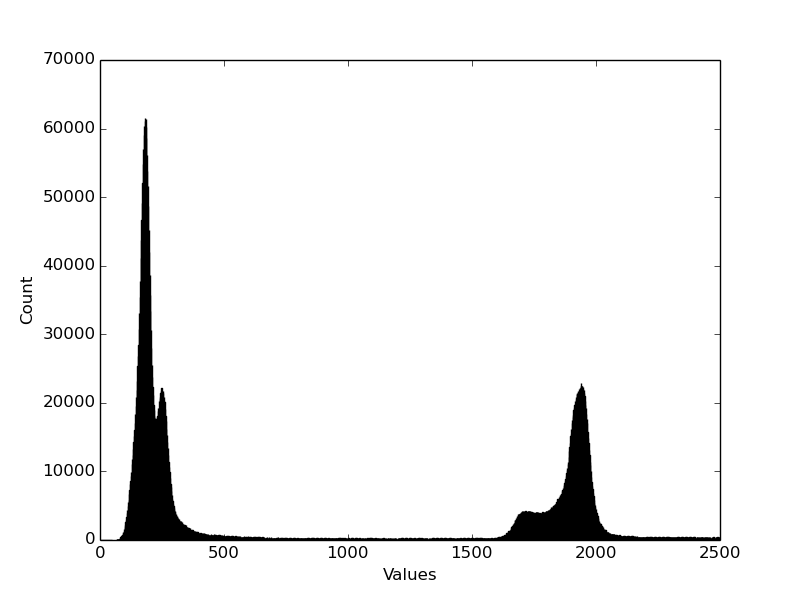
\includegraphics[width=\textwidth]{hist}
\caption{Histogram of the values in the data files}
\label{fig:histLow}
\end{figure}

Based on these distributions of values we have chosen three ranges which we
identify as a) the skin and hair, b) the skeleton head and spine, and c) the
lower jaw, teeth and a strange object in the forehead.

\begin{figure}[h]
	\centering
	\begin{subfigure}[b]{0.3\textwidth}
		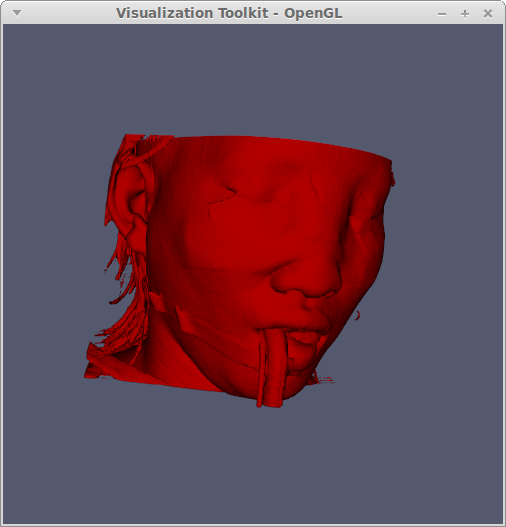
\includegraphics[width=\textwidth]{red}
		\caption{Skin and hair}
		\label{fig:red}
	\end{subfigure}~
	\begin{subfigure}[b]{0.3\textwidth}
		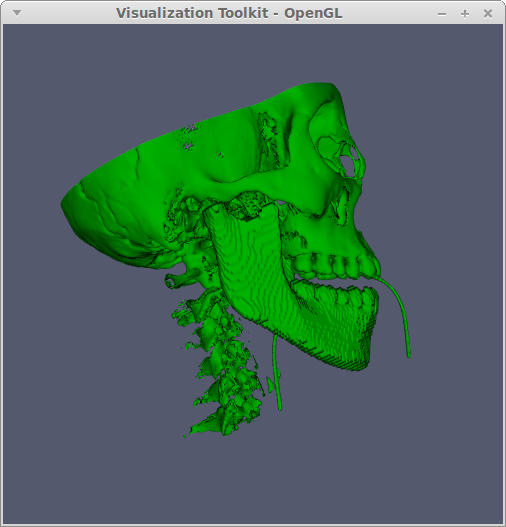
\includegraphics[width=\textwidth]{green}
		\caption{Spine and head}
		\label{fig:green}
	\end{subfigure}~
	\begin{subfigure}[b]{0.3\textwidth}
		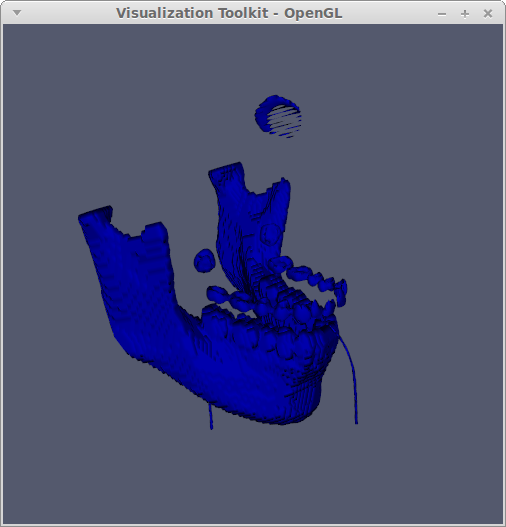
\includegraphics[width=\textwidth]{blue}
		\caption{Jaw and object}
		\label{fig:blue}
	\end{subfigure}
	\caption{The tree ranges}\label{fig:animals}
\end{figure}

These are plotted together in figure \ref{fig:rgb}, each layer is somewhat
transparent in order to show all three of them.

\begin{figure}[h]
	\centering
    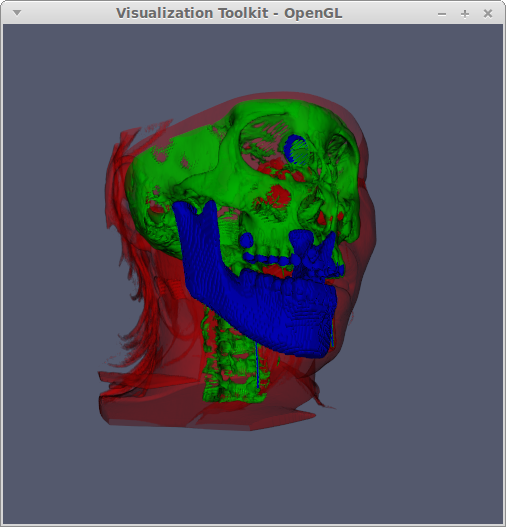
\includegraphics[width=.9\textwidth]{rgb}
    \caption{The three layers}
    \label{fig:rgb}
\end{figure}

We suspect that the cause of that is the strange object in the persons forehead.

Our code can be downloaded from \url{https://github.com/chielk/beautiful\_data}.

\section{Questions and Answers}
\begin{enumerate}
    \item \textit{Identify the correct VTK class capable of reading in a
collection of binary images. There are several that can do this, but some have
features that make it more suitable than others - see the VTK documentation for
more details}

This is the \textsf{vtkImageReader2} class.

    \item \textit{Configure this source stage by invoking the methods of this
class that tell it the specifications of the input data:}

See the source code, specifically the function \textsf{get\_image\_data}.

    \item \textit{Force the source stage to read the dataset by calling its
			\textsf{Update()} method. Now figure out a way to ask the output of
		the source stage for the range of scalar values in the dataset.}

We can do this by calling the methods \textsf{GetScalarTypeMin} and
\textsf{GetScalarTypeMax} on the instance returned by
\textsf{vtkImageReader2.GetOutput()}.

    \item \textit{Add VTK classes to create a visualization pipeline that
renders an isosurface contour of the dataset. Make sure you add an interactor so
that you can interact with the resulting visualization. For the initial contour
value, use a value that is halfway the scalar value range.  Or even better;
allow this value to be passed from the commandline so that you can pass a
different value each time you run your program.}

You can run \textsf{visualize.py}. We have found that halfway the scalar value
range does not yield desirable results. The range for the values are now
hardcodded.

    \item \textit{Tell the contour filter stage to not compute scalar values and
then set a colour in the actor, or}
    \item \textit{Tell the mapper stage to ignore scalar values and then set
a colour in the actor, or}
    \item \textit{Tell the mapper what the actual scalar range is. In this
case the mapper will use a different colour from the red – blue lookup table
depending on the contour value you used.}

We use a different actor for each filtered contour. We set the color and opacity
values for each actor separately.

    \item \textit{Change the background colour. It is also possible to change
the background to a gradient. It’s your choice. Just make sure it does not
interfere with the colours in your visualization. While you are at it: increase
the size of the render window as well.}

We set the background color using the function \textsf{SetBackground} of the
\textsf{vtkRenderer} class. We set the window size using the method
\textsf{SetSize} of the \textsf{vtkRenderWindow} class.

    \item \textit{Experiment with the values for the data spacing and report on
the numbers that you think look appropriate.}

We have set the data spacing to $1 \times 1 \times 2$ to give the head the
proper dimensions.

    \item \textit{Modify your software in order to create a better camera angle
on your visualization.}

The camera position in \textsf{skull.py} has been set to $0 \times 800 \times
500$ to provide a view slightly from the bottom and the front.

    \item \textit{With this new camera angle, it becomes harder to determine the
orientation of the visualization. Add an outline to your visualization that
shows a bounding box to represent the extent of the input data.}

We have created this using the \textsf{vtkOutlineFilter} class.

    \item \textit{Modify your software so that you can visually explore all
contour values in the dataset. You could either use a simple loop to do this, or
if you feel adventurous: add a user interface that supports a slider to set the
contour value interactively. Whatever you use; scan through the visualizations
to detect any anomalies in the data.}

By looking at the histogram, we could identify the points of interest. Using
\textsf{visualize.py} with the \textsf{-c} argument, we conveniently view the
contours at those values to pick the ones we wanted to use for the final
visualization.

    \item \textit{Finally; use the insights obtained from the previous step to
generate one final image that clearly shows the anomaly/lies you found. Make
sure the normal anatomy is also visible so that the anomaly/lies can be seen in
the right context. In your report, describe your approach and your findings.}

See figure \ref{fig:rgb}. We can see that there is a coin-shaped object behind
the patient's brow. The skin shows an indentation at the same angle as the
object (better visible in \ref{fig:red}), and there is a small hole in the bone
bone between the object and the indentation. This suggests that the object
entered through the brow. There is also a tube going into the patient's throat,
but that seems to be inserted as part of the investigation.
\end{enumerate}

\end{document}
